\documentclass[11pt]{article}
\usepackage{amssymb}
\usepackage{tikz}
\usepackage{fancyhdr}
\usepackage{extramarks}
\usepackage{pgfplots}
\usetikzlibrary{automata,positioning}
\usetikzlibrary{shapes.geometric, arrows}


\setlength{\topmargin}{-1.5in}
\setlength{\textheight}{9.5in}
\setlength{\oddsidemargin}{.125in}
\setlength{\textwidth}{6.25in}

\tikzstyle{startstop} = [rectangle, rounded corners, minimum width=3cm, minimum height=1cm,text centered, text width=3cm, draw=black, fill=red!30]
\tikzstyle{basicblock} = [rectangle, minimum width=3cm, minimum height=1cm,text centered, text width=3cm, draw=black, fill=blue!30]

\tikzstyle{io} = [trapezium, trapezium left angle=70, trapezium right angle=110, minimum width=3cm, minimum height=1cm, text centered, text width=2cm,draw=black, fill=blue!30]
\tikzstyle{process} = [rectangle, minimum width=3cm, minimum height=1cm, text centered, text width=2cm,draw=black, fill=orange!30]
\tikzstyle{decision} = [diamond, minimum width=3cm, minimum height=1cm, text centered, text width=2cm, draw=black, fill=green!30]



\tikzstyle{arrow} = [thick,->,>=stealth]
\begin{document}
	\title{
		\textbf{Car Logic Implementation}
	}
	\date{}
	\maketitle

	\begin{tikzpicture}[node distance=2.5cm]



	\node (hardware)[basicblock] {Hardware Sensors};

	\node (autoDriver) [basicblock, below of=hardware] {Autonomous Driver};

	\node (manAgent) [basicblock, below of=autoDriver] {Manufaturer Agent};

	\node (carLogicAPI)[io, below of=manAgent, xshift=3cm]{Car Logic API};

	\node(meshAPI)[io, above of=carLogicAPI, xshift=3cm]{Mesh \\ API};

	\node(netHardware)[basicblock, above of=meshAPI] {Network hardware};



	\draw [arrow] (hardware.250) -- (autoDriver.110);
	\draw [arrow] (autoDriver.70) -- (hardware.290);

	\draw [arrow] (autoDriver.250) -- (manAgent.110);
	\draw [arrow] (manAgent.70) -- (autoDriver.290);

	\draw [arrow] (netHardware.250) -- (meshAPI.110);
	\draw [arrow] (meshAPI.70) -- (netHardware.290);

	\draw [arrow] (meshAPI.250) |- (carLogicAPI.10);
	\draw [arrow] (carLogicAPI.350) -| (meshAPI.290);

	\draw [arrow] (manAgent.290) |- (carLogicAPI.170);
	\draw [arrow] (carLogicAPI.190) -| (manAgent.250);

	\end{tikzpicture}

	\begin{enumerate}
		\item Launchd: Describe here
		\item Sumo: Describe here
		\item Omnet: Describe here
		\item Hardware Simulation: Describe here
		\item Omnet.py: Describe here
	\end{enumerate}
\end{document}
